\documentclass[10pt,a4paper]{article}
%You comment with the modulo-sign. Before the \begin keyword you put what packages
%you want to use etc. If you want to include graphics for example you need the graphicX-package
\usepackage{graphicx}
\usepackage{amsmath}
\usepackage{float}
\usepackage[utf8]{inputenc}
%You also define your title here. You create a title by putting maketitle after you have begun the document
\title{Project Plan}
\author{\begin{large}{Robotics safety}\end{large}\\\\
Olle Fridolfsson (ollfr940) - Responsible Editor\\  Niklas Hansson (nikha310)\\ Patrik Hillgren (pathi747)\\ Benjamin Ingberg (benin542)\\ Pär Lundgren (parlu048)\\ Mattias Nilsson (matni796) - Scrum Master}
\setlength{\parindent}{0cm}	%This removes the automatic indentation
\begin{document}
\maketitle





\centerline{Responsible Editor: Olle Fridolfsson}
%Latex keeps track of your sectioning automatically. To get a table of contents just put
\newpage
\tableofcontents
%To get a new page just put
\newpage
\noindent %Just makes it so that the first paragraph isn't indented
\section{Project Background}
This is a project plan for group ROBOT in the course TSBB11 at Linköping University. TSBB11 is a project course given by the Computer Vision Laboratory where students apply their knowledge from previous theoretical courses in a larger project. The members of the group ROBOT all study the Signal- and Image Processing master program. 
The project assigned to the group is in the area of Robotics Safety and is requested by IEI (Instutitionen för industriell och ekonomisk utveckling/Department of Management and Engineering) at Linköping University and relates to the robot SiA20 Motoman by Yaskawa nordic. 

\section{Project Description}
Robots like Motoman are strong compared to humans. It is therefore important that the robot can detect when humans approach it so that it can take precautions and not hurt anyone. The goal of the project is to be able to determine the distance between the closest moving object and the robot and send a control signal to the robot depending on that information. The control signal should determine four states:

\begin{itemize}
  \item The closest moving object is outside safety zone 2 (see figure below). Objects are not in the collaborative area, the robot can work at standard motion.
  \item The closest moving object is within safety zone 2. This means that the robot motion shall be reduced since the moving object is within the collaborative area.
  \item The closest moving object is within safety zone 1. This means that the robot must stop.
  \item The closest moving object is within emergency zone. This means that the robot must perform an emergency stop, which differs from the usual stop.
\end{itemize}

\begin{figure}[H] 
  \centering
    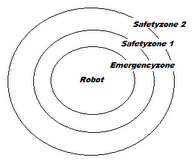
\includegraphics{safetyzones.png}
    \caption{Illustration of safetyzones}
    \label{fig:safetyzone}
\end{figure}

Determining the exact distances of the safety zones is part of the project and it is done according to the SSI ISO standard. Note that the zones are not always circular and that they depend on where the robot is positioned and the orientation the robot is currently in.

\section{Purpose and goal}
The main purpose of this course and this project is being able to solve a problem where the solution requires to apply knowledge from image processing. The project also demands independent work, one of the major goals is to make our own decisions about how we work and what we should work with. This includes defining the method used for developing and the requirements we have on our finished system.

\section{Resources}
Each group member has 240 hours at their disposal split into four sprints,thus giving every sprint 60 hours of work. The physical resources includes the SIA20 Yaskawa Motoman robot, the Yaskawa DX100 controller, Kinect sensors, the possibility to borrow laptops and a room to set up the system. The software will be developed using ROS Industrial.Guidance throughout the project will be available from Johan Hedborg, Postdoc at CVL, and Richard Olsen, PhD student at IEI. 

\section{Limitations}
The result of the project will be limited by the amount of work that can be done in the given time. The visualization of result will not be done in an interactive 3D-environment but in an static 2D-environment. This since the members of the group are more interested in image processing than in computer graphics. A technical limitation will be the cameras field of view. Since the reach of the IR-camera is limited so will the field of view i.e. the visible area around the robot. 

\section{Complexity}
With a possible customer in mind, a system with simple hardware is preferable in order to keep costs down. Having few components is also important to make the installation of the system as easy as possible. If one Kinect sensor does not give sufficient quality, several sensors will be used. However, software will be developed so that it supports a multiple camera setup from the beginning.

\section{Project organization}
We decided that the most suitable way of working is with agile programming where the possibility to make changes is practical and easy. This is mainly because we have had good experience with it before and that we are uncertain on how of details the solution will look like in the end. We choose to work with the software developing method SCRUM, however in a modified way to better adjust to our group and goals. The main difference with our way of working compared to traditional SCRUM is that we will not have an appointed project manager. This is because we are only six members in the group and we will as much as we can work in pairs. Mattias Nilsson will be SCRUM master. Our way of working will be very dynamical and will contain stand up meetings at least two times a week where we go through where we are in the project and what the next step will be. We will also be working in sprints, that is working with predefined problems under 2-3 weeks and then present the so far finished product. After each sprint we will have a sprint retrospective before we start the next iteration, where we evaluate the product and the performed work.
All members of the group has a personal technical area of responsibility. The areas are:

\begin{itemize}
\item Tracking, Benjamin Ingberg
\item Processing robot data (making a 3D model), Pär Lundgren  
\item Robot controlling, Patrik Hillgren
\item Evaluation, Mattias Nilsson
\item Visualisation, Niklas Hansson
\item Merging image data and robot data, Olle Fridolfsson
\end{itemize}

\section{Interested Parties}
The obvious interested parties for this project is IEI, CVL and Yaskawa. But depending on the result it can also be interesting for other companies developing robots. The quality this project will not be dependent on the robot that is used for the development.  

\section{Planning of sprints}
We will be working in sprints that will extend over 2-3 weeks. This gives us the advantage of dividing the working hours more easily and specify what they should contain. Below there is a table showing a rough planning of our sprints, note that there is a possibility that sprints will extend over shorter period of time and therefore the number of sprints will increase.

\subsubsection*{Sprint 1}
\begin{itemize}
  \item Documentation
	\begin{itemize}
	\item Project Plan
	\item System Overview
	\item Design Specification
	\item Document results
	\end{itemize}
	\item Set up
	\begin{itemize}
	\item Install ROS Industrial
	\item Setup communication between the robot and the computer
	\item Setup communication between the Kinect and the computer
	\item Document results
	\end{itemize}
\end{itemize}
\subsubsection*{Sprint 2}
\begin{itemize}
\item Test
\begin{itemize}
\item Calibration between the different coordinate system
\item Process data from robot controller to obtain 3D coordinates
\item Detect moving objects from Kinect data using Background modelling
\item Control robot
\item Try different setups of cameras and robot
\item Document results
\end{itemize}
\end{itemize}
\subsubsection*{Sprint 3}
\begin{itemize}
\item Coding
\begin{itemize}
\item Identify the robot in the image
\item Link robot depth information to the data containing the position of the robot
\item Determine distance from the robot to all other moving objects in the scene
\item Document results
\end{itemize}
\end{itemize}
\subsubsection*{Sprint 4}
\begin{itemize}
\item Refining
\begin{itemize}
\item Speedup and Improvements
\item Technical documentation
\item Design of webpage
\item Evaluation
\item Bug fixing
\end{itemize}
\end{itemize}

\end{document}